%%%%%%%%%%%%%%%%%%%%%%%%%%%%%%%%%%%%%%%%%%%%%%%%%%%%%%%%%%%%%%%%%%%%%%
% Template for a UBC-compliant dissertation
% At the minimum, you will need to change the information found
% after the "Document meta-data"
%
%!TEX TS-program = pdflatex
%!TEX encoding = UTF-8 Unicode

%% The ubcdiss class provides several options:
%%   gpscopy (aka fogscopy)
%%       set parameters to exactly how GPS specifies
%%         * single-sided
%%         * page-numbering starts from title page
%%         * the lists of figures and tables have each entry prefixed
%%           with 'Figure' or 'Table'
%%       This can be tested by `\ifgpscopy ... \else ... \fi'
%%   10pt, 11pt, 12pt
%%       set default font size
%%   oneside, twoside
%%       whether to format for single-sided or double-sided printing
%%   balanced
%%       when double-sided, ensure page content is centred
%%       rather than slightly offset (the default)
%%   singlespacing, onehalfspacing, doublespacing
%%       set default inter-line text spacing; the ubcdiss class
%%       provides \textspacing to revert to this configured spacing
%%   draft
%%       disable more intensive processing, such as including
%%       graphics, etc.
%%

% For submission to GPS
\documentclass[gpscopy,onehalfspacing,11pt]{ubcdiss}
\usepackage[margin=1in,
			left=1.1in]{geometry}
\makeatother


%!TEX root = MJThesis.tex
%%%%%%%%%%%%%%%%%%%%%%%%%%%%%%%%%%%%%%%%%%%%%%%%%%%%%____FONTS___%%%%%
%%
%% FONTS:
%% 
%% The defaults below configures Times Roman for the serif font,
%% Helvetica for the sans serif font, and Courier for the
%% typewriter-style font.  Configuring fonts can be time
%% consuming; we recommend skipping to END FONTS!
%% 
%% If you're feeling brave, have lots of time, and wish to use one
%% your platform's native fonts, see the commented out bits below for
%% XeTeX/XeLaTeX.  This is not for the faint at heart. 
%% (And shouldn't you be writing? :-)
%%
\usepackage[T1]{fontenc}
\usepackage{lettrine}
%% NFSS font specification (New Font Selection Scheme)
\usepackage{times,mathptmx,courier}
\usepackage[scaled=.92]{helvet}
\usepackage{sectsty}
\chapterfont{\usefont{T1}{qhv}{b}{n}\selectfont\huge}
%% Math or theory people may want to include the handy AMS macros
%\usepackage{amssymb}
%\usepackage{amsmath}
% \usepackage[utf8]{inputenc}
% \input{glyphtounicode}
% \pdfgentounicode=1
%\usepackage{amsfonts}
\usepackage{longtable} % fixes issues with the glossary

\usepackage{pifont, fixltx2e} % Adds \textsubscript{}, at least
\usepackage{titlesec} % titles! 
\usepackage[version=3]{mhchem}
\usepackage{float} % Floats! Now can use H as a placement option on floats.
\titleformat{\section}[hang]{
    \usefont{T1}{qhv}{b}{n}\selectfont} % "qhv" - TeX Gyre Heros, "b" - bold
    {} 
    {0em}
    {\hspace{-0.4pt}\Large \thesection\hspace{0.6em}}

%%%%%%%%%%%%%%%%%%%%%%%%%%%%%%%%%%%%%%%%%%%%%%%%%%%%%%____TOC___%%%%%
\usepackage{tocloft} % subfigure option only if using subfigure package
\renewcommand{\cfttoctitlefont} % ToC title
             {\usefont{T1}{qhv}{b}{n}\selectfont\huge}
\renewcommand{\cftchapfont} % chapter titles
             {\usefont{T1}{qhv}{b}{n}\selectfont}
\renewcommand{\cftsecfont} % section titles
             {\usefont{T1}{bch}{m}{n}\selectfont}
\renewcommand{\cftsubsecfont} % subsection titles
             {\usefont{T1}{bch}{m}{n}\selectfont} 
\renewcommand{\cftchappagefont} % chapter page numbers
             {\usefont{T1}{bch}{b}{n}\selectfont}
\renewcommand{\cftsecpagefont} % section page numbers
             {\cftsecfont} 
\renewcommand{\cftsubsecpagefont} % subsection page numbers
             {\cftsubsecfont}
%%%%%%%%%%%%%%%%%%%%%%%%%%%%%%%%%%%%%%%%%%%%%%%%____MICROTYPE___%%%%%
\usepackage[activate={true,nocompatibility},final,tracking=true,kerning=true,spacing=true,factor=1100,stretch=10,shrink=10]{microtype}
% activate={true,nocompatibility} - activate protrusion and expansion
% final - enable microtype; use "draft" to disable
% tracking=true, kerning=true, spacing=true - activate these techniques
% factor=1100 - add 10% to the protrusion amount (default is 1000)
% stretch=10, shrink=10 - reduce stretchability/shrinkability (default is 20/20)
\SetProtrusion{encoding={*},family={bch},series={*},size={6,7}}
              {1={ ,750},2={ ,500},3={ ,500},4={ ,500},5={ ,500},
               6={ ,500},7={ ,600},8={ ,500},9={ ,500},0={ ,500}}
\SetExtraKerning[unit=space]
    {encoding={*}, family={bch}, series={*}, size={footnotesize,small,normalsize}}
    {\textendash={400,400}, % en-dash, add more space around it
     "28={ ,150}, % left bracket, add space from right
     "29={150, }, % right bracket, add space from left
     \textquotedblleft={ ,150}, % left quotation mark, space from right
     \textquotedblright={150, }} % right quotation mark, space from left
\SetExtraKerning[unit=space]
   {encoding={*}, family={qhv}, series={b}, size={large,Large}}
   {1={-200,-200}, 
    \textendash={400,400}}
\SetTracking{encoding={*}, shape=sc}{20}   
\microtypecontext{spacing=nonfrench}        
%%%%%%%%%%%%%%%%%%%%%%%%%%%%%%%%%%%%%%%%%%%%%%%%%%%%%%%%%%%%%%%%%%%%%%
%%
%% Recommended packages
%%
\usepackage{checkend}	% better error messages on left-open environments
\usepackage{graphicx}	% for incorporating external images

%% booktabs: provides some special commands for typesetting tables as used
%% in excellent journals.  Ignore the examples in the Lamport book!
\usepackage{booktabs, multirow}
\usepackage{siunitx, xspace} %for SI units eg. \si{\grams\per\mega\hertz} and gives xspace
\DeclareSIUnit{\molar}{M}  %ugh, now molar works
%% The acro package provides support for defining acronyms, providing
%% their expansion when first used, and building glossaries.  See the
%% example in glossary.tex and the example usage throughout the example
%% document.
%% NOTE: to use \MakeTextLowercase in the \acsfont command below,
%%   we *must* use the `nohyperlinks' option -- it causes errors with
%%   hyperref otherwise.  See Section 5.2 in the ``LaTeX 2e for Class
%%   and Package Writers Guide'' (clsguide.pdf) for details.
\usepackage[single = true, only-used = false]{acro}
%% The ubcdiss.cls loads the `textcase' package which provides commands
%% for upper-casing and lower-casing text.  The following causes
%% the acronym package to typeset acronyms in small-caps
%% as recommended by Bringhurst.
% \renewcommand{\acsfont}[1]{{\scshape \MakeTextLowercase{#1}}}

%% color: add support for expressing colour models.  Grey can be used
%% to great effect to emphasize other parts of a graphic or text.
%% For an excellent set of examples, see Tufte's "Visual Display of
%% Quantitative Information" or "Envisioning Information".
\usepackage{color}
\definecolor{greytext}{gray}{0.5}
%%%%%%%%%%%%%%%%%%%%%%%%%%%%%%%%%%%%%%%%%%%%%%%%%%____COMMENT___%%%%%
%% comment: provides a new {comment} environment: all text inside the
%% environment is ignored.
%%   \begin{comment} ignored text ... \end{comment}
\usepackage{comment}

\titleformat*{\section}{\singlespacing\raggedright\bfseries\Large}
\titleformat*{\subsection}{\singlespacing\raggedright\bfseries\large}
\titleformat*{\subsubsection}{\singlespacing\raggedright\bfseries}
\titleformat*{\paragraph}{\singlespacing\raggedright\itshape}
%%%%%%%%%%%%%%%%%%%%%%%%%%%%%%%%%%%%%%%%%%%%%%%%%%____CAPTION___%%%%%
%% The caption package provides support for varying how table and
%% figure captions are typeset.
\usepackage[format=hang,indention=-1cm,labelfont={bf},margin=1em]{caption}

%% url: for typesetting URLs and smart(er) hyphenation.
%% \url{http://...} 
\usepackage{url}
\urlstyle{sf}	% typeset urls in sans-serif

%%#%#%#%#%#%#%#%#%#%#%#%
%%           Line Numbers!            %%
%%#%#%#%#%#%#%#%#%#%#%#%
\usepackage{lineno}
\linenumbers
% \nolinenumbers  %%#% Comment out to enable line numbers
%!TEX root = MJThesis.tex
%%%%%%%%%%%%%%%%%%%%%%%%%%%%%%%%%%%%%%%%%%%%%%%%%%%%%%%%%%%%%%%%%%%%%%
%% HYPERREF:
%% The hyperref package provides for embedding hyperlinks into your
%% document.  By default the table of contents, references, citations,
%% and footnotes are hyperlinked.
%%
%% Hyperref provides a very handy command for doing cross-references:
%% \autoref{}.  This is similar to \ref{} and \pageref{} except that
%% it automagically puts in the *type* of reference.  For example,
%% referencing a figure's label will put the text `Figure 3.4'.
%% And the text will be hyperlinked to the appropriate place in the
%% document.
%%
%% Generally hyperref should appear after most other packages

%% The following puts hyperlinks in very faint grey boxes.
%% The `pagebackref' causes the references in the bibliography to have
%% back-references to the citing page; `backref' puts the citing section
%% number.  See further below for other examples of using hyperref.
%% 2009/12/09: now use `linktocpage' (Jacek Kisynski): GPS now prefers
%%   that the ToC, LoF, LoT place the hyperlink on the page number,
%%   rather than the entry text.
%% The following is a directive for TeXShop to indicate the main file

\usepackage[hyperref=false,
            url=false,
            isbn=false,
            backref=false,
            firstinits=true,
            style=numeric,
            citereset=chapter,
            maxcitenames=3,
            maxbibnames=100,
            % refsection=section,
            backend=bibtex, % while checking on one of my (newest) systems, this option was needed to generate bibliography
            block=none]{biblatex}

    \usepackage{varioref}

    \usepackage[
		    bookmarksopen=true,
		    linktocpage=true,
		    urlcolor=linkcolor, % Color of URLs
		    citecolor=linkcolor, % Color of citations
		    linkcolor=linkcolor, % Color of links to other pages/figures
		    % backref=page,
		    pdfpagelabels=false,
		    plainpages=false,
		    colorlinks=false, % Turn off all coloring by changing this to false
		    bookmarks=false,
		    pdfview=FitB]{hyperref}

		    %% The following change how the the back-references text is typeset in a
		    %% bibliography when `backref' or `pagebackref' are used
		    % \renewcommand\backrefpagesname{\(\rightarrow\) pages}
		    % \renewcommand\backref{\textcolor{greytext} \backrefpagesname\ }
    %%%%%%%%%%%%%%%%%%%%%%%%%%%%%%
    % Customisation
    %%%%%%%%%%%%%%%%%%%%%%%%%%%%%%
    % back reference text preceding the page number ("see p.")
    \DefineBibliographyStrings{english}{%
        backrefpage  = {see p.}, % for single page number
        backrefpages = {see pp.} % for multiple page numbers
    }

    % the followings activate 'custom-english-ordinal-sscript.lbx'
    % in order to print ordinal 'edition' suffixes as superscripts,
    % and adjusts (reduces) spacing between suffix and following "ed."
    \DeclareLanguageMapping{english}{custom-english-ordinal-sscript}
    \DeclareFieldFormat{edition}%
                       {\ifinteger{#1}%
                        {\mkbibordedition{#1}\addthinspace{}ed.}%
                        {#1\isdot}}

    % removes period at the very end of bibliographic record
    \renewcommand{\finentrypunct}{}

    % removes period after DOI and suppresses capitalization
    % of the word following DOI ("See p. xx" -> "see p. xx")
    \renewcommand{\newunitpunct}{\addspace\midsentence}

    \DeclareFieldFormat{journaltitle}{\mkbibemph{#1},} % italic journal title with comma
    \DeclareFieldFormat[inbook,thesis]{title}{\mkbibemph{#1}\addperiod} % italic title with period
    \DeclareFieldFormat[article]{title}{#1} % title of journal article is printed as normal text
    \DeclareFieldFormat[article]{volume}{\textbf{#1}\addcolon\space} % makes volume of journal bold and adds colon
    \DeclareFieldFormat{pages}{#1} % removes pagination (p./pp.) before page numbers
    %%%%%%%%%
% the command \upcite defined below prints footnote citation above punctuation
\newlength{\spc} % declare a variable to save spacing value
\newcommand{\upcite}[2][]{% new command with two arguments: optional (#1) and mandatory (#2)
        \cite{#2}
        #1% print the optional argument
        }% print (cite) the mandatory argument
%%%%%%%%%
	\usepackage{cleveref}
		\newcommand{\creflastconjunction}{, and\nobreakspace} %Oxford Comma for cref
    %%%%%%%%%
    % the followings activate 'custom-english-ordinal-sscript.lbx'
    % in order to print ordinal 'edition' suffixes as superscripts,
    % and adjusts (reduces) spacing between suffix and following "ed."
    \DeclareLanguageMapping{english}{custom-english-ordinal-sscript}
    \DeclareFieldFormat{edition}%
                       {\ifinteger{#1}%
                       {\mkbibordedition{#1}\addthinspace{}ed.}%
                       {#1\isdot}}    


%\usepackage{longtable}	% provide tables spanning multiple pages
%\usepackage{chngpage}	% support changing the page widths on demand
%\usepackage{tabularx}	% an enhanced tabular environment

%% enumitem: support pausing and resuming enumerate environments.
%\usepackage{enumitem}

%% ragged2e: provides several new new commands \Centering, \RaggedLeft,
%% \RaggedRight and \justifying and new environments Center, FlushLeft,
%% FlushRight and justify, which set ragged text and are easily
%% configurable to allow hyphenation.
%\usepackage{ragged2e}

%% The ulem package provides a \sout{} for striking out text and
%% \xout for crossing out text.  The normalem and normalbf are
%% necessary as the package messes with the emphasis and bold fonts
%% otherwise.
%\usepackage[normalem,normalbf]{ulem}    % for \sout

%% The following commands causes chapter and section references to
%% uppercase the part name.
\renewcommand{\chapterautorefname}{Chapter}
\renewcommand{\sectionautorefname}{Section}
\renewcommand{\subsectionautorefname}{Section}
\renewcommand{\subsubsectionautorefname}{Section}

%% If you have long page numbers (e.g., roman numbers in the 
%% preliminary pages for page 28 = xxviii), you might need to
%% uncomment the following and tweak the \@pnumwidth length
%% (default: 1.55em).  See the tocloft documentation at
%% http://www.ctan.org/tex-archive/macros/latex/contrib/tocloft/
% \makeatletter
% \renewcommand{\@pnumwidth}{3em}
% \makeatother

%%%%%%%%%%%%%%%%%%%%%%%%%%%%%%%%%%%%%%%%%%%%%%%%%%%%%%%%%%%%%%%%%%%%%%
%%%%%%%%%%%%%%%%%%%%%%%%%%%%%%%%%%%%%%%%%%%%%%%%%%%%%%%%%%%%%%%%%%%%%%
%%
%% Some special settings that controls how text is typeset
%%
% \raggedbottom		% pages don't have to line up nicely on the last line
% \sloppy		% be a bit more relaxed in inter-word spacing
% \clubpenalty=10000	% try harder to avoid orphans
% \widowpenalty=10000	% try harder to avoid widows
% \tolerance=1000

%% And include some of our own useful macros
\input{macros}

%%%%%%%%%%%%%%%%%%%%%%%%%%%%%%%%%%%%%%%%%%%%%%%%%%%%%%%%%%%%%%%%%%%%%%
%%%%%%%%%%%%%%%%%%%%%%%%%%%%%%%%%%%%%%%%%%%%%%%%%%%%%%%%%%%%%%%%%%%%%%
%%
%% Document meta-data: be sure to also change the \hypersetup information
%%

\title{The structure, composition, and application of the cell envelope from \textit{Caulobacter crescentus}}
%\subtitle{If you want a subtitle}

\author{Michael D Jones}
\previousdegree{B. Science, Specialization in Biotechnology, University of Alberta, 2006}
\previousdegree{M. Science, Pharmaceutical Sciences, University of Alberta, 2008}

% What is this dissertation for?
\degreetitle{Doctor of Philosophy}

\institution{The University Of British Columbia}
\campus{Vancouver}

\faculty{The Faculty of Science}
\department{Microbiology and Immunology}
\submissionmonth{April}
\submissionyear{2015}

%% hyperref package provides support for embedding meta-data in .PDFlink
%% files
\hypersetup{
  pdftitle={The structure, composition, and application of the cell envelope of \textit{Caulobacter crescentus}  (DRAFT: \today)},
  pdfauthor={Michael D Jones},
  pdfkeywords={Your keywords here}
}

%%%%%%%%%%%%%%%%%%%%%%%%%%%%%%%%%%%%%%%%%%%%%%%%%%%%%%%%%%%%%%%%%%%%%%
%%%%%%%%%%%%%%%%%%%%%%%%%%%%%%%%%%%%%%%%%%%%%%%%%%%%%%%%%%%%%%%%%%%%%%
%% 
%% The document content
%%

%% LaTeX's \includeonly commands causes any uses of \include{} to only
%% include files that are in the list.  This is helpful to produce
%% subsets of your thesis (e.g., for committee members who want to see
%% the dissertation chapter by chapter).  It also saves time by 
%% avoiding reprocessing the entire file.
%\includeonly{intro,conclusions}
%\includeonly{discussion}
\addbibresource{biblio} %%% Bibtex file
\begin{document}

%%%%%%%%%%%%%%%%%%%%%%%%%%%%%%%%%%%%%%%%%%%%%%%%%%
%% From Thesis Components: Tradtional Thesis
%% <http://www.grad.ubc.ca/current-students/dissertation-thesis-preparation/order-components>

% Preliminary Pages (numbered in lower case Roman numerals)
%    1. Title page (mandatory)
\maketitle
%    2. Abstract (mandatory - maximum 350 words)
%% The following is a directive for TeXShop to indicate the main file
%%!TEX root = diss.tex

\chapter{Abstract}

Classically, outer membranes are half lipid, half protein, and the outmost layers of Gram-negative bacteria. For \textit{Caulobacter crescentus} the outer membrane is the penultimate layer beneath protein surface layer (S-layer) composed of the protein RsaA. The caulobacter cell envelope's S-layer is an exciting platform for high density peptide display and biotechnology development. We focused on elucidating the structure of the cell envelope by crystallizing the S-layer protein, RsaA; solving the structure of the the lipopolysaccharide; and functionally characterizing a newly discovered porin, OmpW. 

Bacterial S-layer proteins are highly resistant to crystallization; only two successful examples exist in the literature. Two-dimensional S-layer formation out competes three-dimensional crystal formation. To achieve a crystallisable form of RsaA, a C-terminal truncation version was constructed and expressed in the native host, \textit{C. crescentus}. The secreted protein was prone to aggregation, so low agitation and slow concentration protocols had to be developed. The RsaA truncate produced large crystals that diffracted to <2.5 \AA. Solving the phases proved a serious hurdle. Multiple phaisng strategies were pursued, but the final protein structure remains unsolved.

The lipopolysaccharide of \textit{C. crescentus} is the anchor that supports the S-layer. The structure of the lipid A molecule was solved previously but the structures of the core oligosaccharide and O-polysaccharide had never been deduced. In collaboration with Dr. Evgeny Vinogradov, the remaining unsolved structures in the lipopolysaccharide were solved. The core oligosaccharide has a heptasaccharide structure centering on a rare triple-substituted Kdo residue. The O-polysaccharide is a heptasaccharide containing the dideoxy sugar N-acetylperosamine. Additionally, a previously unknown rhamnan polysaccharide was discovered and its structure was determined. 

Porins, non-specific passive protein channels, are significant components of classical Gram-negative outer membranes. Despite this, no porin had ever been identified in the \textit{C. crescentus}. Here we report the identification and characterization of the porin OmpW in \textit{C. crescentus}.  OmpW has low conductance of 125 pSv in 1 M KCl, this is interesting because the homologous porins in other bacteria have no detectable pore-forming activity.

The cell envelopes of bacteria are remarkable structures; the work in thesis presents new information about the unique structures in the caulobacter envelope. 

	\cleardoublepage

%    3. Preface
%% The following is a directive for TeXShop to indicate the main file
%%!TEX root = diss.tex

\chapter{Preface}
\begin{epigraph} 
\textit{``Plenum ingenni pudoris fateri per quos profeceris''}\\
(To own up to those who were the means of one's own achievements)\\
Pliny the Elder, Natural History
\end{epigraph} 

The contents contained herein are original work by or in collaboration with me,
the primary author, unless specified below.

\paragraph{Chapter 2} 
Portions of chapter 2 have been used for the preparation of a manuscript for
submission for publication. The work was done in collaboration with Dr.\,Anson
Chan. I preformed all the experiments and wrote the wrote the majority of the
manuscript. Dr.\,Chan assisted in the X-ray diffraction data collection, the
data evaluation and processing, and edited and provided feedback on the writing
of the manuscript. 

\paragraph{Chapter 3}
Portions of chapter 3 have been published; \fullcite{jones2015core}. The work was
done as a collaboration with Dr.\,Evgeny Vinogradov. Dr.\,Vinogradov was
responsible for the majority of the structural work: monosaccharide analysis,
methylation analysis, and \textsc{NMR} analysis, as well as the written
summaries of those methods. Dr.\,John Nomellini constructed the strain used,
JS1025. The cytokine and cell culture experiments were new additions not present
in any publication. The execution of the HEK-Blue assay was performed by Gyles Ifill. I was
responsible for the preparation of all the samples, experimental design, and
writing the manuscript. 

\paragraph{Chapter 4}
A version of chapter 4 has been submitted for publication. I was responsible for
the sample preparation, purification, and strain construction. The laboratory of
Dr.\,Roland Benz was responsible for synthetic membrane conductance experiments.
The writing was a split collaboration.
	\cleardoublepage

%    4. Table of contents (mandatory - list all items in the preliminary pages
%    starting with the abstract, followed by chapter headings and
%    subheadings, bibliographies and appendices)
\tableofcontents
	\cleardoublepage	% required by tocloft package

%    5. List of tables (mandatory if thesis has tables)
\listoftables
	\cleardoublepage	% required by tocloft package

%    6. List of figures (mandatory if thesis has figures)
\listoffigures
	\cleardoublepage	% required by tocloft package

%    7. List of illustrations (mandatory if thesis has illustrations)
%    8. Lists of symbols, abbreviations or other (optional)

%    9. Glossary (optional)
%% The following is a directive for TeXShop to indicate the main file
%%!TEX root = diss.tex

\DeclareAcronym{LPS}{
short = lps,long = lipopolysaccharide, 
short-format = \scshape}
\DeclareAcronym{PS}{
short = ps,long = polysaccharide, 
short-format = \scshape}
\DeclareAcronym{OPS}{
short = ops,long = O-specific polysaccharide, 
short-format = \scshape}
\DeclareAcronym{OS}{
short = os,long = oligosaccharide, 
short-format = \scshape}
\DeclareAcronym{UV}{
short = uv,long = ultraviolet Light, 
short-format = \scshape}
\DeclareAcronym{MALDI-TOF}{
short = maldi-tof,long = matrix assisted laser desorption/ionization-time of flight mass spectroscopy, 
short-format = \scshape}
\DeclareAcronym{S-layer}{
short = S-layer,long = protein surface layer, 
short-plural = {s}}
\DeclareAcronym{GC-MS}{
short = gc-ms,long = gas chromatography-mass spectroscopy, 
short-format = \scshape}
\DeclareAcronym{NMR}{
short = nmr,long = nuclear magnetic resonance spectroscopy, 
short-format = \scshape}
\DeclareAcronym{SDS-PAGE}{
short = sds-page,long = sodium dodecyl sulfate-polyacrylamide gel electrophoresis, 
short-format = \scshape}
\DeclareAcronym{PBS}{
short = pbs,long = phosphate-buffered saline, 
short-format = \scshape}
\DeclareAcronym{EDTA}{
short = edta,long = ethylenediaminetetraacetic acid, 
short-format = \scshape}
\DeclareAcronym{COSY}{
short = cosy,long = correlation spectroscopy, 
short-format = \scshape}
\DeclareAcronym{OD600}{
    short = \textsc{od}$_{600}$ ,
    long = optical density at 600 \si{\nano\metre} 
}
\DeclareAcronym{PCR}{
    short = pcr ,
    long = polymerase chain reaction, 
    short-format = \scshape 
}
\DeclareAcronym{gCOSY}{
short = g\textsc{cosy}, long = gradient correlation spectroscopy}
\DeclareAcronym{TOCSY}{ 
short = tcosy, long = total correlation spectroscopy,
short-format = \scshape}
\DeclareAcronym{PC}{
    short = pc,
    long = phosphatidylcholine, 
    short-format = \scshape}
\DeclareAcronym{ROESY}{
short = roesy,long = rotating frame nuclear Overhauser effect spectroscopy, 
short-format = \scshape}
\DeclareAcronym{HSQC}{
short = hsqc,long = heteronuclear single quantum coherence, 
short-format = \scshape}
\DeclareAcronym{gHSQC}{
short = g\textsc{hsqc}, long = gradient heteronuclear singe quantum coherence}
\DeclareAcronym{HMBC}{
short = hmbc,long = heteronuclear multiple bond coherence, 
short-format = \scshape}
\DeclareAcronym{gHMBC}{
short = g\textsc{hmbc}, long = gradient heteronuclear multiple bond coherence}
\DeclareAcronym{NOE}{
short = noe,long = nuclear Overhauser enhancement, 
short-format = \scshape}
\DeclareAcronym{NOESY}{
short = noesy, long = nuclear Overhauser enhancement spectroscopy, 
short-format = \scshape}
\DeclareAcronym{HMQC}{
short = hmqc,long = heteronuclear multiple-quantum correlation spectroscopy,
short-format = \scshape}
\DeclareAcronym{TLC}{
short = tlc,long = thin-layer chromatography, 
short-format = \scshape}
% \DeclareAcronym{ABC}{
% short = abc,long = ATP-binding cassette, 
% short-format = \s
% cshape}
\DeclareAcronym{EPS}{
short = eps,long = extracellular polysaccharide, 
short-format = \scshape}
\DeclareAcronym{PYE}{
    short = pye,
    long = peptone-yeast extract medium, 
    short-format = \scshape}
\DeclareAcronym{LDAO}{
    short = ldao ,
    long = lauryldimethylamine-oxide, 
    short-format = \scshape}
\DeclareAcronym{ESI}{
short = esi,long = electrospray ionization, 
short-format = \scshape}
\DeclareAcronym{TFA}{
short = tfa,long = trifluoroacetic acid, 
short-format = \scshape}
\DeclareAcronym{caulobacter}{
    short = C.\,crescentus,
    long = \textit{Caulobacter crescentus}, 
    short-format = \textit,
    class = bacteria
}
\DeclareAcronym{ecoli}{
    short = E.\,coli,
    long = \textit{Escherichia coli}, 
    short-format = \textit,
    class = bacteria
}
\DeclareAcronym{pseudomonas}{
    short = P.\,aeruginosa ,
    long = \textit{Pseudomonas aeruginosa} ,
    short-format = \textit,
    class = bacteria
}
 %%%%%%%--------------Sugars
\DeclareAcronym{man}{
    short = Man,
    long = mannose, 
    class = sugar
}
\DeclareAcronym{rha}{
    short = Rha ,
    long = rhamnose , 
    class = sugar
}
\DeclareAcronym{per}{
    short = PerN,
    long = perosamine , 
    class = sugar
}
\DeclareAcronym{glc}{
    short = Glc,
    long = glucose, 
    class = sugar
}
\DeclareAcronym{glca}{
    short = GlcA,
    long = glucuronic acid, 
    class = sugar
}
\DeclareAcronym{glcnac}{
    short = GlcNAc ,
    long = N-acetylglucosamine , 
    class = sugar
}
\DeclareAcronym{gala}{
    short = GalA,
    long = galacturonic acid, 
    class = sugar
}
\DeclareAcronym{hep}{
    short = Hep,
    long = heptose,
    class = sugar
}
\DeclareAcronym{glcome}{
    short = 3-O-MeGlc,
    long = 3-O-methylglucose, 
    class = sugar
}
\DeclareAcronym{MS}{
    short = ms,
    long = mass spectrometry, 
    short-format = \scshape
} 
\DeclareAcronym{kdo}{
    short = Kdo,
    long = ketodeoxyoctulosonic acid, 
    class = sugar
}
\DeclareAcronym{blast}{
    short = blast,
    long = Basic Local Alignment Search, 
    short-format = \scshape 
}
\DeclareAcronym{aa}{
    short = aa,
    long = amino acid, 
    short-format = \scshape 
}
\DeclareAcronym{cls}{
    short = cls,
    long = Canadian Light Source, 
    short-format = \scshape 
}
\DeclareAcronym{ssrl}{
    short = ssrl,
    long = Stanford Synchotron Radiation Light Source , 
    short-format = \scshape 
}
\DeclareAcronym{rtx}{
    short = rtx,
    long = repeat-in-toxin, 
    short-format = \scshape 
}
\DeclareAcronym{peg}{
    short = peg,
    long = polyethylene glycol, 
    short-format = \scshape 
}
\DeclareAcronym{mw}{
    short = mw,
    long = molecular weight, 
    short-format = \scshape 
}
\DeclareAcronym{pi}{
    short = pI,
    long = isoelectric point, 
}
\DeclareAcronym{t1ss}{
    short = t1ss ,
    long = type 1 secretion system, 
    short-format = \scshape 
}
\DeclareAcronym{abc}{
    short = abc ,
    long = \textsc{atp} binding cassette, 
    short-format = \scshape 
}
\DeclareAcronym{kd}{
    short = $K_D$ ,
    long = dissociation constant 
}
\DeclareAcronym{anthrax}{
    short = B.\,anthracis ,
    long = \textit{Bacillus anthracis}, 
    short-format = \itshape , 
    class = bacteria
}
\DeclareAcronym{aeromonas}{
    short = A.\,salmonicida ,
    long = \textit{Aeromonas Salmonicida}, 
    short-format = \itshape , 
    class = bacteria
}
\DeclareAcronym{cfetus}{
    short = C.\,fetus,
    long = \textit{Campylobacter fetus}, 
    short-format = \itshape , 
    class = bacteria
}
\DeclareAcronym{cfg}{
    short = cfg,
    long = Consortium of Functional Glycomics, 
    short-format = \scshape 
}
\DeclareAcronym{dls}{
    short = dls ,
    long = dynamic light scattering, 
    short-format = \scshape 
} 
\DeclareAcronym{salmonella}{
     short = S. typhimurium ,
    long = \textit{Salmonella typhimurium}, 
    short-format = \itshape , 
    class = bacteria
}
\DeclareAcronym{pma}{
    short = pma ,
    long = phorbol 12-myristate 13-acetate, 
    short-format = \scshape 
}
\DeclareAcronym{tnfa}{
    short = tnf-$\alpha$ ,
    long = tumor necrosis factor $\alpha$, 
    short-format = \scshape 
}
\DeclareAcronym{il}{
    short = il ,
    long = interleukin, 
    short-format = \scshape 
}
\DeclareAcronym{mcp1}{
    short = mcp-1 ,
    long = monocyte chemotactic protein 1, 
    short-format = \scshape 
}
\DeclareAcronym{ifnb}{
    short = ifn-$\beta$ ,
    long = interferon $\beta$, 
    short-format = \scshape
}
\DeclareAcronym{geo}{
    short = G. staerothermophilus ,
    long = \textit{Geobacillus stearothermophilus}, 
    short-format = \itshape , 
    class = bacteria
}	% always input, since other macros may rely on it
	\textspacing		% begin one-half or double spacing

%   10. Acknowledgements (optional)
%% The following is a directive for TeXShop to indicate the main file
%%!TEX root = diss.tex

\chapter{Acknowledgments}

First and most of all I'd like to thank my family. My parents, J.C. and Dorothea, your support has been completely indispensable. I am lucky to have such fantastic parents. My wife, Elizabeth, I started this PhD before I met you but I couldn't have finished it without you. 

I do believe I have had the best supervisory committee of anyone I know. Dr.\,Beatty, Dr.\,Murphy, and  Dr.\,Fernandez you have been the exactly perfect level of supportive, critical, and congratulatory. Thank you.

I have been incredibly fortunate to have been in the Smit lab. It has been said that choosing your supervisor is the most important choice you have to make in grad school---I chose well in John Smit. Dr.\,Smit, your patience with my crazy ideas let me grow as a scientist but your lack of patience with my crazy ideas kept me in line and prevented my PhD from lasting a decade. Dr.\,Nomellini, I have been fortunate to have you nearby to fix my mistakes, hear me complain about my mistakes, and showing me how to prevent future mistakes. The few other members of our lab that I have shared time with, Lyngrace, Jan, Christina, you have all been great allies in the lab.

Beyond the official credits that the are given, I want to acknowledge the incredible collaborators I have had since day one. 
Dr.\,Evgeny Vinogradov is the world's preeminent expert on bacterial polysaccharide analysis, there is quite literally no one that would have been a better collaborator for our lipopolysaccharide work. The Consortium for Functional Glycomics Core H at Emory Univeristy were incredibly easy to work with and even though our results with them were ultimately negative, the service they provide is an invaluable asset to the field. Dr.\,Martine Caroff has been a surprisingly helpful source of expertise and critique, especially critique.

The Murphy lab in our department of Microbiology and Immunology is the go to collaborators for protein X-ray crystallography, my experiences are evidence to why that is. All of them (Angele, Meghan, Slade, Jason, Catherine, Stephanie, Marek, Michael, Mariko) accepted me like a lab member from the start. Dr.\,Anson Chan was an exceptional partner for crystallography, his expertise kept us moving forward against a tough project. Especially I would like to thank Dr.\,Chan for staying up all night many times on our long data collection runs. Staying up late isn't so bad, but staying up late for poor results deserves commendation. 

Dr.\,Roland Benz was my only collaborator to initiate a collaboration with us. The porin project started as a side-project but it has become a nice little story that I am happy to have been apart of. Dr.\,Benz, I hope to actually meet you one day.

Lastly, I would like to acknowledge my department as a whole. This department has been incredibly supportive and warm. I feel with people like Darlene, Sue, and Dr.\,Gold guiding the ship, I never felt like we were going to crash. A special acknowledgment goes to Dr.\,Jan Burian, who was always around with encouragement and advice but especially for his organization of many departmental events and teams that brought together a cadre of scientists on the dodgeball court, on the softball diamond, and beyond the confines of campus.



%   11. Dedication (optional)

% Body of Thesis (not all sections may apply)
\mainmatter

	\acresetall	% reset all acronyms used so far

%    1. Introduction
%% The following is a directive for TeXShop to indicate the main file
%!TEX root = ../MJThesis.tex
\acresetall

\chapter{Introduction}
\label{ch:Introduction}

\begin{epigraph}
    \emph{But during the writing of this review, I learned how little I knew in this area, and this was a humbling and sobering experience. I am certain that I have made many mistakes due to my ignorance, and I hope that the review will be useful despite its many faults} ---~Hiroshi Nikaido (2003), my grand supervisor.
\end{epigraph}

\section{History of S-layers} % (fold)
\label{sec:history_of_s_layers}
   

    \begin{figure}[p] % First S-layer
            \begin{center}
                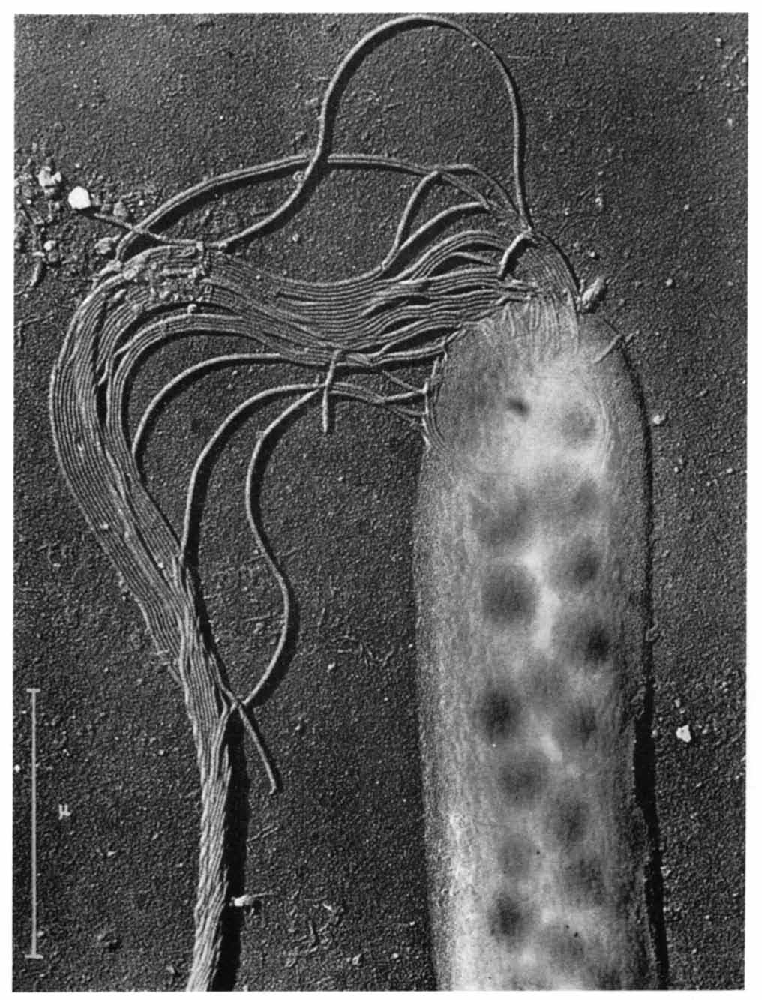
\includegraphics[]{intro/img/firstslayer.pdf}
            \end{center}
            \caption[The first published image of a \ac{S-layer}.]{The first published image of a \ac{S-layer}. The hexagonal \ac{S-layer} on the surface of the bacterium --- probably \textit{Spirillum} sp. --- is visible along the edges of the cell body (centre right). The scale bar denotes one micrometre. (This image is Fig. 1 from \fullcite{firstslayer} )}
            \label{fig:firstslayer}
    \end{figure}
    
    \begin{figure}[p]
        \begin{center}
            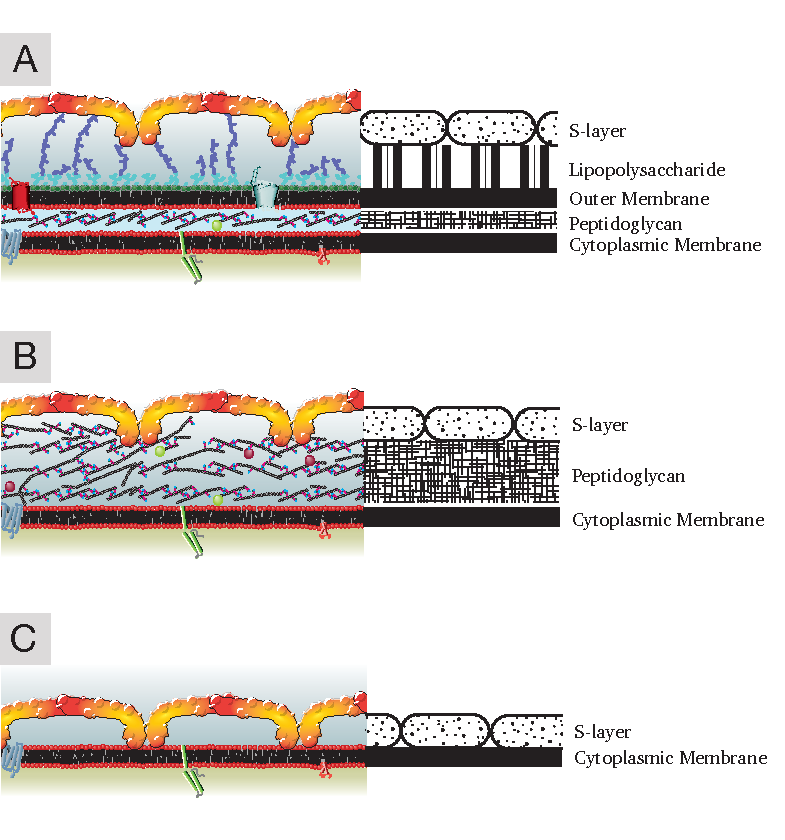
\includegraphics[]{intro/img/celwalls.pdf}
        \end{center}
        \caption[Cross-sectional diagrams of the cell envelopes]{Cross-sectional diagrams of the cell envelopes of (\textbf{A}) Gram negative bacteria, (\textbf{B}) Gram positive bacteria, and (\textbf{C}) archaebacteria. In all known cases the \ac{S-layer} sits on the extreme outer surface of the cell. (This diagram was inspired by Fig. 1 from \fullcite{sleytr1983crystalline})}
        \label{fig:cellwalls}
    \end{figure}
% section history_of_s_layers (end)


\endinput

Any text after an \endinput is ignored.
You could put scraps here or things in progress.


%    2. Main body
% Generally recommended to put each chapter into a separate file
%% The following is a directive for TeXShop to indicate the main file
%!TEX root = ../MJThesis.tex

\chapter{The core and O-polysaccharide structure of the \textit{Caulobacter crescentus} lipopolysaccharide}
\label{ch:lps}

\section{Introduction} % (fold)
\label{sec:introduction} 
	\textit{Caulobacter crescentus} is an aquatic alphaproteobacterium well known for a stalked, crescent cell morphology, asymmetric cell division, and a \ac{S-layer}. \caulobacter is a widely studied model organism for cell development and differentiation; despite this, the structure of its lipopolysaccharide (\ac{LPS}) has not yet been fully determined.

	Interest in the \ac{LPS} of \caulobacter is focused on its immunological profile \upcite{caulobacterlipida} and its structural role as an anchor for the self-assembled, paracrystalline protein S-layer \upcite{walker94}. The \ac{LPS} of \caulobacter possesses a much reduced immunogenic activity, most likely due to its lipid A structure, which is significantly different from that of \ac{LPS} from enteric bacteria. The lipid A structure has been reported \upcite{caulobacterlipida}; it is a unique molecule containing a di-diaminoglucose backbone (instead of di-glucosamine) and two galacturonate moieties that replace the canonical phosphates that are on each end of the disaccharide in most lipid A molecules. The \caulobacter \ac{S-layer} non-covalently attaches to the \ac{OPS} \upcite{walker94}. However, the \ac{OPS} structure has not been resolved. Genetic analyses have pointed towards the unusual N-acetylperosamine being a major component \upcite{awramgenes}. A notable feature of this O-antigen is that it exists completely hidden beneath the S-layer, presumably inaccessible to the environment \upcite{walker94}. Carbohydrate structures from non-pathogenic bacterial \ac{LPS} are rarely studied and an \ac{LPS} that is sequestered beneath an \ac{S-layer} is not represented in the literature.

	In the present study our data has determined the core oligosaccharide structure from \caulobacter CB15 NA1000, (advancing an earlier report of core composition \upcite{ravenscroftlps}) as well as the central backbone and non-reducing ends of its OPS. Unexpectedly, we identified a previously unknown rhamnan polysaccharide. Along with previous reports on lipid A \upcite{caulobacterlipida} and \ac{EPS} \upcite{ravenscrofteps}, we believe the major carbohydrate structures in \caulobacter cell envelope have now been solved.
% section introduction (end)

\section{Results} % (fold)
\label{sec:results}

	\subsection{Initial assessment and component analysis} % (fold)
	\label{sub:initial_assessment_and_component_analysis}

		The \ac{PS} was released from the \ac{LPS} by hydrolysis with acetic acid. 1H \ac{NMR} spectrum of the \ac{PS} (Fig. 1) contained a large number of partially overlapping signals of various intensities in the anomeric region. It was obviously not a regular polymer with well-defined repeating units. Attempts to separate this material by anion-exchange chromatography led to the isolation of a number of fractions from neutral to slightly retained, but all of them had virtually identical \ac{NMR} spectra. Methylation of the polysaccharide led to the identification of 3- and 3,4-substituted mannopyranose, terminal glucopyranose (derived from side-chain 3-O-methyl-glucose), terminal, 3-, 4-, and 2,4-substituted rhamnopyranose, 3-substituted Rha4NAc, and an unidentified derivative resembling methylated Rha4N that eluted between dimethylhexose derivatives and 3-substituted Rha4NAc. To identify the position of the methyl groups in naturally methylated monosaccharides, methylation was conducted with \ce{CD3I}. This confirmed the identification of tetramethylglucitol as originating from 3-O-methyl-glucose, but did not identify any other naturally methylated monosaccharides, visible in \ac{NMR} spectra. An unknown derivative received two deuterated methyl groups.
	% subsection initial_assessment_and_component_analysis (end)

	\subsection{O-Antigen structure determination (PS1)} % (fold)
	\label{sub:o_antigen_structure_determination_ps1_}

		A set of 2D spectra (\ac{gCOSY}, \ac{TOCSY}, \ac{NOESY}, 1H-13C \ac{gHSQC}, \ac{gHMBC}, \ac{gHSQC}-\ac{TOCSY}) was obtained for the \ac{PS}. There were many (more than 20) lines of correlations from the anomeric signals. Later, after the analysis of \ac{PS} degradation products, most of them could be assigned to particular structures (Fig. 2). Polysaccharide heterogeneity was not caused by random acetylation, but \ac{PS} contained 4 methyl groups (one major and 3 minor). Monosaccharide analysis revealed L-Rha, D-Man, D-Rha4N (perosamine), and 3-O-methyl-D-glucose. Other methylated monosaccharides were not identified by GC-MS as alditol acetates, possibly due to low content or degradation during hydrolysis.

		In an attempt to simplify the structure, \ac{PS} was oxidized with \ce{NaIO4}, reduced with NaBD4, hydrolyzed with 2\% \ce{AcOH}, and the products were separated on a Biogel P6 column to give a polymer and an oligosaccharide 1 (\ac{OS}1). Analysis of \ac{OS}1 will be described below. For some reason not all of the rhamnan was oxidized, and some of its signals persisted in the spectra of the remaining polymer (without side-chain Rha F). To remove the rest of it, the oxidation was repeated to produce \ac{PS}1. Spectra still contained some signals of minor components, analyzed later. Assignment of the spectra of the non-oxidizable polymer \ac{PS}1 was difficult due to complete or partial overlap of the H-2,3,4,5 signals of Rha4NAc. To improve signal spread, \ac{PS}1 was deacylated with 4M \ce{NaOH}. At this point the major polymer became positively charged and an attempt was made to separate it from the minor components using cation-exchange chromatography. However, all material was eluted together at high salt concentration, thus indicating that all components were chemically bound together. Assignment of the spectra (Fig. 3, Table 1) became possible at this stage due to better signal spread (H-4 signals of Rha4N moved to high field due to deacylation) and the sequence shown on the Fig. 2 was proposed. Spectra contained the signals of two β-mannopyranose, 3-O-Me-$\alpha$-Glcp, and two -Rhap4N. The following interresidual \ac{NOE} and \ac{HMBC} correlations were used to determine the sequence: R1:L3, L1:Z3, Z1:Q3, Q1:W3, W1:X3, A1:X4. \ac{PS}1 had trisaccharide repeating units composed of $\beta$-mannose and two $\alpha$-Rha4NAc residues, and every second repeating unit carried a side branch of 3-O-Me-Glc. It seems that side-chains were present quite regularly at each second trisaccharide repeat of the main chain, because \ac{NOE} correlations were observed between the repeating units with and without 3-OMe-Glc, and not between units of the same structure. Thus altogether, the repeating unit contained seven monosaccharides.
	% subsection o_antigen_structure_determination_ps1_ (end)

	\subsection{Minor component determination} % (fold)
	\label{sub:minor_component_determination}

		 \ac{PS} and \ac{PS}1 spectra contained signals of minor components, which could not be removed by chromatography, as described above. They probably represented the non-reducing ends of the major chain, \ac{PS}1 (Fig. 2). The minor components contained methylated Rha (2-O-Me-Rha residue J and 2,3-Me2-Rha4N residue B). The position of the methyl groups were found from \ac{HMBC} correlations between protons of methyl groups and carbon atoms bearing OMe groups, which all were well visible and did not overlap with other signals due to their low field position. Thus, two independent structural fragments, 1 and 2, were found and are shown in the Fig. 2. Mannose residues Z' and Z" at the non-reducing ends of these fragments were further linked to Rha4N residues, indistinguishable from the Rha4N of the main chain. Rha4N residue D had upfield shifted C-2 and downfield shifted C-3 signals (Table 2), which have not been explained. It appears that its O-3 was phosphorylated, producing typical phosphorylation signal shifts and broadening of the H-3 signal, but 1H-31P \ac{HMQC} \ac{NMR} spectrum showed no signals, possibly due to the low abundance of this residue. Possibly Rha residues inserted in the structure resembling PS1 represented the attachment point of the rhamnan (PS2) to \ac{PS}1, if they were linked together.
	% subsection minor_component_determination (end)

	\subsection{Rhamnan polysaccharide determination (PS2)} % (fold)
	\label{sub:rhamnan_polysaccharide_determination_ps2_}

		Periodate oxidation of the \ac{PS} produced an \ac{OS}1, which was analyzed by \ac{NMR} and its structure, as shown on Fig. 2, was determined using standard 2D \ac{NMR} methods. Signal assignment is shown in the Table 3. It contained three rhamnopyranose units and 4-deoxy-1-deutero-erythritol, produced by the oxidation-reduction of 4-substituted rhamnose. Formation of this oligosaccharide could be explained by oxidation of the side chain Rha F and 4-substituted Rha G in the \ac{PS}1 (letter labels for monosaccharides were given using anomeric signals in the whole \ac{PS} spectra starting from low-field). The unoxidized 4-substituted residue T in the oligosaccharide originally carried side-chain Rha F at position 2. Knowing the \ac{OS}1 structure the signals of a corresponding polymer (\ac{PS}2) were identified in the spectra of the whole \ac{PS}, and are given in the Table 3. 
	% subsection rhamnan_polysaccharide_determination_ps2_ (end)

	\subsection{Core oligosaccharide determination} % (fold)
	\label{sub:core_oligosaccharide_determination}

		The core oligosaccharide of the \caulobacter{} \ac{LPS} isolated after AcOH hydrolysis contained one non-degraded Kdo, two LD-Hep, one DD-Hep, mannose, galactose, and glucuronic acid in pyranose form. 2D \ac{NMR} analysis led to the structure shown on Fig. 2 (\ac{NMR} assignments are in the Table 4, \ac{HSQC} spectrum Fig. 4). The sequence followed from the observed \ac{NOE}: E1:C5,C7,F5; F1:E2; G1:F3; H1:C7,E2; K1:C4; L1:K4. Correlation E1:C7 is always observed in the α-Hep-5-Kdo fragment. E1:F5 was due to the -Man-2-Hep linkage. H1E2 indicates spatial proximity of the residues E and H, linked to the same Kdo C. All expected transglycoside correlations were observed in \ac{HMBC} spectrum, together with intra-ring correlations H-1:C-3 and H-1:C-5 for all α-pyranoses. Methylation analysis revealed terminal DD-Hep, terminal and 2-substituted LD-Hep, 3-substituted Man and terminal Gal. The structure agreed with mass spectral data, \ac{ESI} negative [M-H]- = 1314.9, [M-2H]/2- = 656.7, calculated exact mass Hex2Hep3HexA1Kdo1 = 1314.4 Da. 
	% subsection core_oligosaccharide_determination (end)
% section results (end)

\section{Methods} % (fold)
\label{sec:methods}

	\subsection{Bacterial strain construction and growth conditions} % (fold)
	\label{sub:bacterial_strain_construction_and_growth_conditions}

		The strain used for the preparation of \ac{LPS} was JS1025, a derivative of \caulobacter CB15 NA1000. The salient features are that it has an engineered amber mutation in \textit{rsaA} leading to the loss of the \ac{S-layer} and the gene CCNA\_00471 has been inactivated by a partial deletion. CCNA\_00471 encodes a putative GDP-L-fucose synthase \upcite{na1000genome}. The knockout (\del 471) confers a deficiency in an \ac{EPS} that was previously found to contain L-fucose \upcite{ravenscrofteps}. CCNA\_00471 was disrupted in the same manner as previously in JS4038 \upcite{hivmicrobicide2}, except the starting strain used here was JS1023 \upcite{slayercryo}. 
		
		Cells were grown to mid-to-late log phase (\od = 0.9) in M16HIGG defined medium at 30\cel in 2.8 \si{\litre} Fernbach flasks containing 1250 \millilitre of medium, shaking at 100 rpm. M16HIGG is a modification of M6HIGG medium \upcite{smitpilin81}, containing 0.31\% glucose, 0.09\% glutamate, 1.25 \si{\milli\meter} sodium phosphate, 3.1 \si{\milli\meter} imidazole, 0.05\% ammonium chloride and 0.5\% modified Hutner's Mineral Base \upcite{hutners}. 
	% subsection bacterial_strain_construction_and_growth_conditions (end)

	\subsection{\texttt{LPS} isolation} % (fold)
	\label{sub:LPS_isolation}

		\ac{LPS} was isolated from the cells via disrupting the outer membrane by chelation. The protocol was a modification of the procedure reported by Walker \etal \upcite{walker94}. Cells were centrifuged at 12 400 x g for 10 min. The pellets were suspended with distilled water and recentrifuged. These pellets were resuspended in 1/10 original culture volume in \ac{PBS} \upcite{maniatis} amended with 35 \si{\milli\meter} \ac{EDTA}, agitated at room temperature for 10 min and then centrifuged at 15 300 x g for 15 min. The supernatant was retrieved and re-centrifuged, as before, to ensure clarity and then dialyzed against 5 \si{\milli\meter} \ce{MgCl2}. DNase and RNase were added to final concentrations of 10 \si{\micro\gram\per\milli\litre} and 100 \si{\micro\gram\per\milli\litre}, respectively, and incubated at 37\cel for 2 h. Proteinase K was added to a final concentration of 0.3 \mgperml and the preparation was incubated at 50\cel overnight. The sample was then ultracentrifuged at 184 000 x g for 3 h. Glassy pellets formed which were suspended in distilled water to 1/100 original culture volume. A Bligh-Dyer extraction was performed to reduce contaminating lipids \upcite{blighdyer}.
	% subsection \ac{LPS}_isolation (end)

	\subsection{Gel electrophoresis} % (fold)
	\label{sub:gel_electrophoresis}

		Discontinuous \ac{SDS-PAGE} was performed with a 13\% separating gel \upcite{laemmli}. Detection of \ac{LPS} was done by periodate oxidation and silver staining as described by Zhu \etal \upcite{improvedsilverstain}.
	% subsection gel_electrophoresis (end)

	\subsection{\texttt{NMR} spectroscopy} % (fold)
	\label{sub:nmr_spectroscopy}

		\ac{NMR} experiments were carried out on a Varian INOVA 600 \si{\mega\hertz} (1H) spectrometer with 5 \si{\milli\meter} gradient probe at 25--50\cel with acetone internal reference (2.225 ppm for 1H and 31.45 ppm for 13C), using standard pulse sequences \ac{gCOSY}, \ac{TOCSY}(mixing time 120 \si{\milli\second}), \ac{ROESY} (mixing time 300 \si{\milli\second}),  \ac{gHSQC}, and  \ac{gHMBC}(100 \si{\milli\second} long range transfer delay), \ac{HMQC} for \textsuperscript{1}H-\textsuperscript{31}P correlation, JHX set to 10 \si{\hertz}. AQ time was kept at 0.8--1 sec for H-H correlations and 0.25 sec for \ac{HSQC}. 256 increments were acquired for t1 in all 2D spectra, except 512 for \ac{gCOSY}.
	% subsection nmr_spectroscopy (end)

	\subsection{Chromatography} % (fold)
	\label{sub:chromatography}

		Gel chromatography was performed on a Sephadex G-15 column (1.5x60 cm) or a Bio-gel P6 column (2.5x60 cm) in pyridine-acetic acid buffer (4 \millilitre:10 \millilitre:1 \si{\litre} water), and monitored by refractive index detector (Gilson). Anion exchange chromatography was done on an Hitrap Q column (2x5 \millilitre size, Amersham), with \ac{UV} monitoring at 220 nm in a linear gradient of \ce{NaCl} (0--1 M, 1 h) at the 3 \si{\milli\litre\per\minute}. Fractions of 1 min were collected and additionally tested for carbohydrates, by spotting on an \ce{SiO2} \ac{TLC} plate, dipping them in 5\% \ce{H2SO4} in \ce{EtOH} and heating with a heat-gun. All fractions of interest were dried in a Savant drying centrifuge and 1H spectra were recorded for each fraction without desalting. For 2D \ac{NMR}, desalting was performed on a Sephadex G15 column. 
	% subsection chromatography (end)

	\subsection{Monosaccharide analysis} % (fold)
	\label{sub:monosaccharide_analysis}

		Samples with added inositol standard were hydrolyzed with 3 M \ac{TFA} at 120 \cel. Monosaccharides were converted to alditol acetates by conventional methods and identified by \ac{GC-MS} on a Varian Saturn 2000 instrument on a DB17 capillary column (30 m x 0.25 \si{\milli\meter} ID x 0.25 \si{\micro\meter} film) with helium carrier gas, using a temperature gradient 170\cel (3 min), 250\cel at 5\si{\degreeCelsius\per\minute}.
	% subsection monosaccharide_analysis (end)

	\subsection{Determination of absolute configurations of monosaccharides} % (fold)
	\label{sub:determination_of_absolute_configurations_of_monosaccharides}

		To the polysaccharide sample (0.2 \milligram) (R)-2-\ce{BuOH} (0.2 \millilitre) and acetyl chloride (0.02 \millilitre) were added at room temperature, heated at 90 \cel for 2 h, dried by air stream, acetylated, analyzed by \ac{GC-MS} as described above. Standards were prepared from monosaccharides of known configuration with (R)- and (S)-2-\ce{BuOH}.
	% subsection determination_of_absolute_configurations_of_monosaccharides (end)

	\subsection{Methylation analysis} % (fold)
	\label{sub:methylation_analysis}

		For the methylation analysis core sample (2 \milligram) was dephosphorylated with 50 \microlitre of 48\% \ce{HF} for 20 h at +10\cel, diluted with 2 \millilitre of ethanol, precipitate collected by centrifugation, washed with 2 \millilitre of ethanol, dried.

		Methylation was performed by Ciucanu-Kerek procedure \upcite{ciucanufrancisc}. 0.5 \milligram of the sample was dissolved in 0.5 \millilitre of dry DMSO with heating at 100 \cel for 5-10 min until complete dissolution. Powdered \ce{NaOH} (about 50 \milligram) was added and the mixture was stirred for 30 min. 0.2 \millilitre of MeI was added and the mixture was stirred for a subsequent 30 min. The sample was then flushed with air to remove the MeI and diluted to 10 \millilitre with water. The sample was passed through a C18 Seppak cartridge, washed with 10 \millilitre of water, and then the methylated compound was eluted with 5 \millilitre of methanol. The methylated product was hydrolyzed with 3 M TFA (120 \cel, 3h), dried, reduced with \ce{NaBD4}, and the reagent destroyed with 0.5 \millilitre of 4 M \ce{HCl}. The solution was dried under a stream of air and dried twice more with the addition of \ce{MeOH} (1 \millilitre). The sample was acetylated with 0.4 \millilitre \ce{Ac2O} and 0.4 \millilitre pyridine for 30 min at 100\cel. It was then dried and analyzed by \ac{GC-MS}.
	% subsection methylation_analysis (end)

	\subsection{Periodate oxidation} % (fold)
	\label{sub:periodate_oxidation}

		 \ac{PS} (10 \milligram) was dissolved in water (2 \millilitre). \ce{NaIO4} (20 \milligram) was added and the solution was incubated at room temperature for 24 h. Ethylene glycol (0.2 \millilitre) and an excess \ce{NaBD4} were added. The solution was then kept for 1 h before being treated with 0.2 \millilitre of \ce{AcOH} and desalted on a Sephadex G-15 column. The product was hydrolyzed with 2\% \ce{AcOH}, 2 h at 100\cel, and  separated on a Sephadex G-50 column to give \ac{OS}1.
	% subsection periodate_oxidation (end)

% section methods (end)

\section{Discussion} % (fold)
\label{sec:discussion}

	The \ac{LPS} of \caulobacter has an unusually complicated structure with two different polysaccharides, irregular substituents, and unfavourable \ac{NMR} spectra. Presented data show structures of the core part, two polymers, and putative terminal structures. The polysaccharides could not be separated by size exclusion or anion-exchange chromatography and are probably linked together through the same core. The core of the \caulobacter{} \ac{LPS} has been studied previously and an initial assessment of its composition was made \upcite{ravesncroftlps}, but the complete structure had not been determined. The structure of the \ac{OPS} has not been studied before. In our view the polysaccharide structure of the C. crescentus \ac{LPS} represents one of the most complicated bacterial \ac{LPS} polysaccharide structures identified so far.

	The Kdo present in the \ac{LPS} core structure (Fig. 2) has the typical substitutions at O-4 and O-5 of a manno-configured sugar and a negatively charged sugar, respectively \upcite{brade99}. It also has a rarely observed third substitution at O-7 with a heptose moiety. The Kdo O-7 position is known to be occupied by a galactose moiety in the core of \textit{Rhizobium leguminosarum} bv. Viciae VF39 \upcite{rhizobiumlps}, and the secondary Kdo in the core oligosaccharide from \textit{Acinetobacter baumannii} ATCC 19606 has an O-7 substituted with a glucosamine \upcite{acinetobacterlps}. 

	In the traditional model \ac{LPS} occupies the outer leaflet of the outer membrane of a Gram-negative bacterium, and so (excepting the presence of cell associated \ac{EPS}) is the outermost layer of the cell. For \caulobacter, however, \ac{LPS} is the penultimate barrier below the protein \ac{S-layer}. The \caulobacter{} \ac{OPS} serves as the anchor for the S-layer and is likely not accessible to the environment \upcite{walker94}. The carbohydrates found in the OPS are particularly hydrophobic, marked by the abundance of deoxy-sugars, acetyl groups, and methyl groups. This hydrophobicity is possibly a result of particular sugars needed for \ac{S-layer} anchoring, as these carbohydrate structures likely evolved as the cognate ligands for the \ac{S-layer} protein, RsaA. The distance between the \ac{S-layer} and the outer membrane is about 17--19 nm \upcite{dipm}. It is possible the hydrophobicity aids in packing the polysaccharides between the S-layer and the \ac{LPS}. Further determination of RsaA's structure should help illuminate the interaction between the S-layer and \ac{OPS}.

	Knowledge of the structure of \caulobacter{}�� \ac{OPS} and \ac{LPS} will facilitate the determination and characterization of their biosynthetic enzymes and mutant variants. Already, the enzymes LpxI \upcite{lpxi} and GDP-L-perosamine acetylase \upcite{perosmineacetyltransferase} from \caulobacter have been characterized. One uncharacterized enzyme, WbqL, is necessary for proper \ac{OPS} synthesis and disruption of wbqL leads to the accumulation of truncated and S-layer anchoring deficient \ac{OPS} in the inner membrane and inhibits Crescentin-mediated cell curvature \upcite{lpsinterferecrescentin}. Many genes, such as wbqL, have been identified as essential for \ac{OPS} synthesis \upcite{awramgenes} but have not yet been characterized. Other genes, that must be essential for \ac{OPS} synthesis, have yet to be identified or characterized, such as the O-antigen polymerase and ligase.

	% --Should I increase the text about lpxI?--%

	The subunit-based repeating nature of \caulobacter{}�� \ac{OPS} suggests that a Wzy-dependent pathway synthesizes the polymer \upcite{lpsreview}. The previous study that aimed to identify genes essential for \ac{OPS} did not identify many of the canonical genes in the Wzy-dependant pathway \upcite{awramgenes}, such as the O-unit transporter, Wzx, O-antigen polymerase, Wzy; the chain-length determinate protein, Wzz; and the O-antigen ligase, WaaL. Genes that have been annotated as putative O-antigen synthesis genes do appear in the sequenced genomes for \caulobacter CB15, but they have not been experimentally confirmed. 

	An additional aspect to this \ac{LPS} it the fact that its O-antigen is of homogenous length. While other \ac{LPS}s vary in size due to the number of O-antigen repeat groups, appearing as a laddering of bands by \ac{SDS-PAGE}, the \ac{LPS} from C. crescentus appears as a single band \upcite{walker94}. Initial \ac{MALDI-TOF} analysis of the entire \ac{LPS} indicates a size of about 10.8 kDa (not shown).  % Must show! %
	After accounting for the solved structures for the lipid A and core regions, this suggests the \ac{LPS} contains approximately 5 repeats of the proposed heptameric O-antigen structure.  There is not currently a known mechanism for the regulation and synthesis of a strictly homogenous length O-antigen. It is possible that this \ac{OPS} is synthesized via the \ac{ABC}-transporter-dependent pathway \upcite{lpsreview} or another heretofore undiscovered mechanism. In any event it would seem that the transfer of a polysaccharide of this considerable size to the outer leaflet of the outer membrane is a remarkable feat for the bacterium.
 
% section discussion (end)


% Table 1. \ac{NMR} data for Caulobacter crescentus main polysaccharide PS1 (40 \cel) and deacylated PS2 (50 \cel). Me at 3.62/61.3 ppm.

% Table 4. \ac{NMR} data for the minor components of the double oxidized non-deacylated \ac{PS} (50 \cel). Methyl group signals: B2: 3.48/59.5; B3: 3.42/57.9; J2: 3.45/59.6 ppm (H/C).

% Table 3. \ac{NMR} data for C. crescentus polysaccharide PS2 and its NaIO4 oxidation product OS1 (40 \cel).

% Table 4. \ac{NMR} data for the core oligosaccharide (25\cel).
 
% Fig. 1. 1H \ac{NMR} spectra of the intact C. crescentus O-specific polysaccharide (bottom trace), double oxidized polysaccharide (middle trace) and N-deacylated double oxidized polysaccharide (upper trace).

% Fig. 2. The structures of Caulobacter crescentus polysaccharides, their derivatives, core oligosaccharide, and minor components. 

% Fig. 3. Overlap of COSY (green), TOCSY (red) and ROESY (black) correlations from anomeric protons of double oxidized deacylated C. crescentus polysaccharide PS1.

% Fig. 4. Fragment of 1H-13C HSQC spectrum of the core.


%\include{model}
%\include{impl}
%\include{discussion}
%\include{conclusions}
%    3. Notes
%    4. Footnotes
%    5. Bibliography
% prints author names as small caps
\renewcommand{\mkbibnamefirst}[1]{\textsc{#1}}
\renewcommand{\mkbibnamelast}[1]{\textsc{#1}}
\renewcommand{\mkbibnameprefix}[1]{\textsc{#1}}
\renewcommand{\mkbibnameaffix}[1]{\textsc{#1}} 
\printbibliography[heading=bibintoc]

\appendix
%    6. Appendices (including copies of all required UBC Research
%       Ethics Board's Certificates of Approval)
%\include{reb-coa}	% pdfpages is useful here
\chapter{Supporting Materials}
\section{The amino acid sequence of RsaA from \caulobacter}
\label{app:rsaseq}
\texttt{\underline{MAYTTAQLVTAYTNANLGKAPDAATTLTLDAYATQTQTGGLSDAAALTNTLKLVNSTTAV}\hfill-60~~\\
\underline{AIQTYQFFTGVAPSAAGLDFLVDSTTNTNDLNDAYYSKFAQENRFINFSINLATGAGAGA}\hfill-120~\\
\underline{TAFAAAYTGVSYAQTVATAYDKIIGNAVATAAGVDVAAAVAFLSRQANIDYLTAFVRANT}\hfill-180~\\
\underline{PFTAAADIDLAVKAALIGTILNAATVSGIGGYATATAAMI}NDLSDGALSTDNAAGVNLFT\hfill-240~\\
AYPSSGVSGSTLSLTTGTDTLTGTANNDTFVAGEVAGAATLTVGDTLS\textbf{GGAGTDVLN}WVQ\hfill-300~\\
AAAVTALPTGVTISGIETMNVTSGAAITLNTSSGVTGLTALNTNTSGAAQTVTAGAGQNL\hfill-360~\\
TATTAAQAANNVAVDGGANVTVASTGVTSGTTTVGANSAASGTVSVSVANSSTTTTGAIA\hfill-420~\\
VTGGTAVTVAQTAGNAVNTTLTQADVTVTGNSSTTAVTVTQTAAATAGATVAGRVNGAVT\hfill-480~\\
ITDSAAASATTAGKIATVTLGSFGAATIDSSALTTVNLSGTGTSLGIGRGALTATPTANT\hfill-540~\\
LTLNVNGLTTTGAITDSEAAADDGFTTINIAGSTASSTIASLVAADATTLNISGDARVTI\hfill-600~\\
TSHTAAALTGITVTNSVGATLGAELATGLVFT\textbf{GGAGADSILL}GATTKAIVMGAGDDTVTV\hfill-660~\\
SSATLGAGGSVN\textbf{GGDGTDVLV}ANVNGSSFSADPAFGGFETLRVAGAAAQGSHNANGFTAL\hfill-720~\\
QLGATAGATTFTNVAVNVGLTVLAAPTGTTTVTLANATGTSDVFNLTLSSSAALAAGTVA\hfill-780~\\
LAGVETVNIAATDTNTTAHVDTLTLQATSAKSIVVTGNAGLNLTNTGNTAVTSFDASAVT\hfill-840~\\
GTGSAVTFVSANTTVGEVVTIR\textbf{GGAGADSLT}GSATANDTII\textbf{GGAGADTLV}YTGGTDTFT\textbf{G}\hfill-900~\\
\textbf{GTGADIFD}INAIGTSTAFVTITDAAVGDKLDLVGISTNGAIADGAFGAAVTLGAAATLAQ\hfill-960~\\
YLDAAAAGDGSGTSVAKWFQFGGDTYVVVDSSAGATFVSGADAVIKLTGLVTLTTSAFAT\hfill-1020\\
EVLTLA\hfill-1026}
 
This would be any supporting material not central to the dissertation.
For example:
\begin{itemize}
\item Authorizations from Research Ethics Boards for the various
    experiments conducted during the course of research.
\item Copies of questionnaires and survey instruments.
\end{itemize}



\backmatter
%    7. Index
% See the makeindex package: the following page provides a quick overview
% <http://www.image.ufl.edu/help/latex/latex_indexes.shtml>


\end{document}
